\chapter{Edge Connectivity}
Sia $G=(V,E)$ un grafo non orientato connesso. L'\textbf{edge-connectivity} di $G$ è il \textbf{minimo} numero di archi che occorre rimuove da G affinché il grafo sia disconnesso.
\begin{figure}[H]
    \centering
    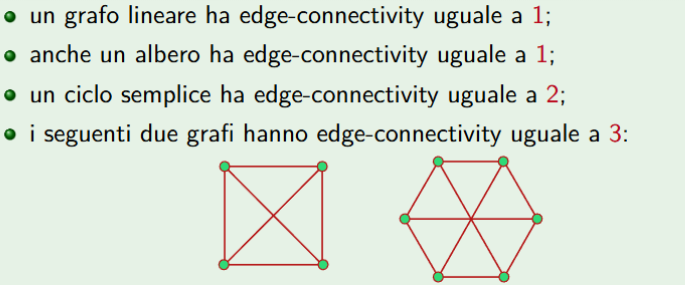
\includegraphics[width=0.5\linewidth]{Images/edge_connectivity/esempi.png}
\end{figure}
Un \textbf{insieme di disconnessione} per $G$ è un insieme minimale $D \subseteq E$ di archi di $G$ tale che $(V, E - D)$ sia disconnesso.
Indichiamo con $Disconn(G)$ la collezione di tutti gli insiemi di disconnessione per G. Avremo che $edge-connectivity(G) = min |D|$.

Definiamo un \textbf{Taglio} in $G=(V,E)$ è un partizione non banale $|\langle V_1, V_2 \rangle|$ di $V$ tale che nessuno degli insiemi è vuoto. La \textbf{dimensione} del taglio è data dal numero di archi che lo attraversano cioè:
\[|\langle V_1, V_2 \rangle| = |\{(u,v) \in V_1 \times V_2: (u, v) \in G\}|\]

\section*{Lemma 1}
Sia $D\subseteq E$ un insieme di disconnessione per un grafo connesso $G=(V,E)$, allora:
\begin{enumerate}
    \item Il sottografo $(V, E - D)$ ha esattamente due componenti connesse.
    \item Il taglio in $G$ introdotto da $D$ è attraversato da tutti e soli gli archi in $D$.
\end{enumerate}
\begin{figure}[H]
    \centering
    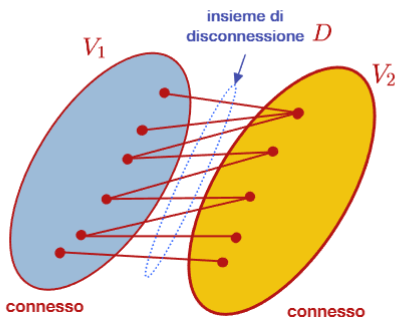
\includegraphics[width=0.4\linewidth]{Images/edge_connectivity/insieme_di_disconnessione.png}
\end{figure}
Si consideri un arco qualunque $e \in D$, poiché:
\begin{itemize}
    \item $(V, E - D)$ non è connesso.
    \item $(V, (E - D) \cup \{e\})$ è connesso per via della minimalità di D. (e il grafo rimanesse rotto anche dopo aver rimesso $e$, vorrebbe dire che $e$ non serviva a nulla per rompere il grafo)
\end{itemize}
Ne consegue che $(V, E - D)$ è formato da 2 componenti connesse. Siano $(V_1, E_1)$ e $(V_2, E_2)$ le due componenti connesse, il taglio $|\langle V_1, V_2 \rangle|$ indotto da D non è attraversato alcun arco in $E - D$. Dunque il taglio è attraversato tutti e soli dagli archi di D.

Sappiamo che ogni insieme di disconnessione minimale ($D$) crea un taglio perfetto, attraversato esattamente dagli archi di $D$. Di conseguenza, se ogni disconnessione è un taglio, allora la dimensione del taglio più piccolo possibile ($\min |\langle V_1, V_2 \rangle|$) non può essere più grande della disconnessione più piccola ($\min |D|$). Dunque:
\[\min Taglio \leq \min Disconnesione\]
Viceversa, se prendiamo un taglio qualsiasi. Gli archi che attraversano questo taglio separano il grafo. Magari ne hai presi troppi (non è minimale), ma sicuramente dentro quel mucchio di archi c'è un sottoinsieme che basta a disconnettere il grafo. Di conseguenza, a disconnessione più piccola possibile ($\min |D|$) deve essere per forza più piccola o uguale a quel mucchio di archi del taglio. Dunque:
\[\min Disconnesione \leq \min Taglio\]
Pertanto $\min Taglio = \min Disconnessione$ e, dunque, l'edge connectivity del grafo è uguale al minimo taglio possibile.

Dato un grafo non orientato $G$, indichiamo $\bar{G}$ il grafo orientato ottenuto da G introducendo due archi orientati opposti al posto dell'arco non orientato. Una volta fatto ciò, possiamo definire la \textbf{rete unitaria} inserendo $c(u, v)= 1$ per ogni arco nel grafo $\bar{G}$. 
\section*{Lemma 2}
Sia $G=(V,E)$ un grafo non orientato connesso e sia $|\langle V_1, V_2 \rangle|$ un taglio in $G$. Siano $s,t \in V$ tali che $s \in V_1$ e $t \notin V_2$ e sia $(\bar{G}, s, t, c)$ la rete unitaria indotta da $G, s$ e $t$, allora:
\[|\langle V_1, V_2 \rangle| = c(V_1,V_2) = c(V_2,V_1)\]
In pratica, il numero di archi fisici che tagli nel grafo originale ($|\langle V_1, V_2 \rangle|$) è esattamente uguale alla capacità matematica del taglio nella nuova rete di flusso ($c(V_1, V_2)$).
Per dimostrarlo, siano:\footnote{Giuro che è l'ultima dimostrazione}
\[e_1 = (v_{11}, v_{12}), \dots, e_k = (v_{k1}, v_{k2})\]
gli archi di $G$ che attraversano il taglio. Allora:
\begin{align*}
    |\langle V_1, V_2 \rangle| = k \\
    c(V_1, V_2) = \sum_{i=1}^{k} c(v_{i1},v_{i2}) = k\\
    c(V_2, V_1) = \sum_{i=1}^{k} c(v_{i2},v_{i1}) = k
\end{align*}
Da cui la tesi.
\section*{Lemma 3}
Sia $G=(V,E)$ un grafo non orientato e sia $s \in V$. Esiste $t \in V - \{s\}$ per cui la rete unitaria indotta da $G$ ha un taglio minimo la cui capacità eguaglia l'edge connectivity di $G$. 
\textit{Dimostrazione}\footnote{Mentivo}\\
Sia $\langle V_1, V_2 \rangle$ un taglio di dimensione minima in $G$ di dimensione uguale alla edge connectivity di $G$. Supponiamo che $s$ sia in $V_1$ e $t \in V_2$. Allora $(V_1,V_2)$ è un taglio della rete unitaria la cui capacità è uguale alla dimensione del taglio $\langle V_1, V_2 \rangle$ in $G$, pertanto $(V_1,V_2)$ è un taglio minimo. 
\begin{figure}[H]
    \centering
    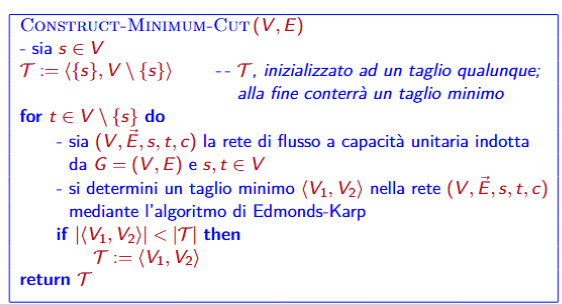
\includegraphics[width=0.5\linewidth]{Images/edge_connectivity/minimum_cut.png}
\end{figure}

Dunque, per ciascuna esecuzione dell'algoritmo \textbf{Edmonds-Karp} nel ciclo for, richiede al più $|V|$ incrementi di flusso, dunque ha complessità $O(VE)$. Poiché vi sono complessivamente $|V|-1$ esecuzioni di Edmonds-Karp, Construct Minimum Cut ha complessità $O(V^2E)$. 